%% This is file `elsarticle-template-1-num.tex',
%%
%% Copyright 2009 Elsevier Ltd
%%
%% This file is part of the 'Elsarticle Bundle'.
%% ---------------------------------------------
%%
%% It may be distributed under the conditions of the LaTeX Project Public
%% License, either version 1.2 of this license or (at your option) any
%% later version.  The latest version of this license is in
%%    http://www.latex-project.org/lppl.txt
%% and version 1.2 or later is part of all distributions of LaTeX
%% version 1999/12/01 or later.
%%
%% The list of all files belonging to the 'Elsarticle Bundle' is
%% given in the file `manifest.txt'.
%%
%% Template article for Elsevier's document class `elsarticle'
%% with numbered style bibliographic references
%%
%% $Id: elsarticle-template-1-num.tex 149 2009-10-08 05:01:15Z rishi $
%% $URL: http://lenova.river-valley.com/svn/elsbst/trunk/elsarticle-template-1-num.tex $
%%
\documentclass[preprint,12pt]{elsarticle}

%% Use the option review to obtain double line spacing
%% \documentclass[preprint,review,12pt]{elsarticle}

%% Use the options 1p,twocolumn; 3p; 3p,twocolumn; 5p; or 5p,twocolumn
%% for a journal layout:
%% \documentclass[final,1p,times]{elsarticle}
%% \documentclass[final,1p,times,twocolumn]{elsarticle}
%% \documentclass[final,3p,times]{elsarticle}
%% \documentclass[final,3p,times,twocolumn]{elsarticle}
%% \documentclass[final,5p,times]{elsarticle}
%% \documentclass[final,5p,times,twocolumn]{elsarticle}

%% if you use PostScript figures in your article
%% use the graphics package for simple commands
%% \usepackage{graphics}
%% or use the graphicx package for more complicated commands
%% \usepackage{graphicx}
%% or use the epsfig package if you prefer to use the old commands
%% \usepackage{epsfig}

%% The amssymb package provides various useful mathematical symbols
\usepackage{amssymb}
%% The amsthm package provides extended theorem environments
%% \usepackage{amsthm}

%% The lineno packages adds line numbers. Start line numbering with
%% \begin{linenumbers}, end it with \end{linenumbers}. Or switch it on
%% for the whole article with \linenumbers after \end{frontmatter}.
%% \usepackage{lineno}

%% natbib.sty is loaded by default. However, natbib options can be
%% provided with \biboptions{...} command. Following options are
%% valid:

%%   round  -  round parentheses are used (default)
%%   square -  square brackets are used   [option]
%%   curly  -  curly braces are used      {option}
%%   angle  -  angle brackets are used    <option>
%%   semicolon  -  multiple citations separated by semi-colon
%%   colon  - same as semicolon, an earlier confusion
%%   comma  -  separated by comma
%%   numbers-  selects numerical citations
%%   super  -  numerical citations as superscripts
%%   sort   -  sorts multiple citations according to order in ref. list
%%   sort&compress   -  like sort, but also compresses numerical citations
%%   compress - compresses without sorting
%%
%% \biboptions{comma,round}

% \biboptions{}


\journal{Science of Computer Programming}

\usepackage{hyperref}
\usepackage{color}

\newcommand{\definition}[1]{ 
\begin{quote} \item {\em #1} \end{quote}}
\newcommand {\chaptersummary}[1] { \vspace{3cm} \hrule \vspace{0.5cm} {\em #1 } \vspace{0.5cm} \hrule \vspace{0.5cm} \newpage}
\newcommand{\challenge}[1]{\paragraph {\bf \em [Challenge]} {\em #1}} 



\newcommand{\chapquote}[1]{\em #1} 


\newcommand{\quest}[1]{{\em ({\bf Mircea:} #1)}}
\newcommand{\mir}[1]{{\em ({\bf Mircea:} #1)}}
\newcommand{\mircea}[1]{{\em ({\bf Mircea:} #1)}}
\newcommand{\Mircea}[1]{{\em ({\bf Mircea:} #1)}}

\newcommand{\pg}[2]{#1 #2}
%\newcommand{\pg}[2]{\paragraph {#1} {\small #2}}
\newcommand{\mic}[1]{{\small #1}}

\definecolor{lg}{rgb}{0.9,0.9,0.9}
\definecolor{darkblue}{rgb}{0.0,0.0,0.5}


\newcommand{\cbar}{\vspace {1cm} \hrule }

\newcommand{\concls}[1]{\titlebox{Facts and Limitations}{#1}}

\newcommand{\titlebox}[2]{
\vspace{1cm}
\hrule
\vspace{0.25cm}
{\bf #1: }
\vspace{0.25cm}
\hrule
#2
\vspace{0.5cm}
}


% Utils

\newcommand{\dpdef}[1]{\paragraph{Definition.} {\em #1}}
\newcommand{\dpdisc}[1]{\paragraph {Discussion.} #1}
\newcommand{\dpr}[1]{\paragraph {Rationale.} #1}
\newcommand{\dpcat}[1]{\paragraph {Category:} #1}
\newcommand{\dpcatage}{\dpcat{Age-related}}
\newcommand{\dpcatdyn}{\dpcat{Dynamics-related}}
\newcommand{\dpexample}[1]{\paragraph {Example.} #1}
\newcommand{\dpp}[1]{\newpage\subsection{#1}}


\newcommand{\pidea}[1]{#1.}
\newcommand{\pideap}[1]{#1}
%\newcommand{\pidea}[1]{\paragraph{#1.}}
%\newcommand{\pideap}[1]{\paragraph{#1} }



\newcommand{\flabel}[1]{\label{fig:#1}}
\newcommand{\tlabel}[1]{\label{tab:#1}}
\newcommand{\clabel}[1]{\label{c:#1}}
\newcommand{\slab}[1]{\label{sec:#1}}

\newcommand{\fref}[1]{Figure \ref{fig:#1}}
\newcommand{\tref}[1]{Table \ref{tab:#1}}
\newcommand{\sref}[1]{Section \ref{sec:#1}}
\newcommand{\cref}[1]{Section \ref{c:#1}}

% Font conventions
\newcommand{\partref}[2]{{\bf Part \ref{p:#1}: #2}}
\newcommand{\chap}[1]{\item {\bf Chapter \ref{c:#1}} {\footnotesize (p.\pageref{c:#1})}}
\newcommand{\apdx}[1]{\item {\bf Appendix \ref{c:#1}} {\footnotesize (p.\pageref{c:#1})}}
\newcommand{\spref}[1]{Section \ref{sec:#1} {\footnotesize (p.\pageref{sec:#1})}}

\newcommand{\SOC}{\subsubsection* {Structure of the Chapter}}

\newcommand{\q}[1]{``#1''}

\newcommand{\tool}[1]{{\em #1}}
\newcommand{\pnam}[1]{{\em #1}}
\newcommand{\trm}[1]{{\em #1}}

\newcommand{\art}[1]{{\em #1}}
\newcommand{\book}[1]{{\em #1}}
\newcommand{\cit}[1]{{\em ``#1''}}

\newcommand{\proj}[1]{{\em #1}}
\newcommand{\dev}[1]{{\em #1}}
\newcommand{\term}[1]{{\em #1}}
\newcommand{\class}[1]{{\em #1}}
\newcommand{\method}[1]{{\em #1}}
\newcommand{\met}[1]{{\em #1}}
\newcommand{\pack}[1]{{\em #1}}
\newcommand{\model}[1]{{\em #1}}
\newcommand{\vp}[1]{{\em #1}}

\newcommand{\metric}[1]{{\em #1}}

\newcommand{\cod}[1]{{\em #1}}



% Tables with metrics
\newcommand{\metrictableh}[4]{
\begin{table}[h!]
%\footnotesize
\centering
\begin{tabular}{l l}
#1
\hline
#2
\hline
\end{tabular}
\caption{#3}\tlabel{#4}
\end{table}
}

\newcommand{\metrictable}[3]{
\metrictableh
{Acronym & Name\\}{#1}{#2}{#3}
}




% viewpoint definitions
\newcommand{\vpc}{black}
\newcommand{\Goal}[1]{\subsubsection* {Goal} #1}
\newcommand{\Cat}[1]{\subsubsection* {Category} #1}

\newcommand{\Concerns}[1]{\paragraph{\textcolor{\vpc}{Concerns}} \begin{itemize}#1\end{itemize}}
\newcommand{\Stakeholders}[1]{\paragraph{\textcolor{\vpc}{Stakeholders: }} #1}
\newcommand{\Construction}[1]{\subsubsection* {Construction Principles } #1}
\newcommand{\Navigation}[1]{\paragraph{\textcolor{\vpc}{Implementation in SPO.}}  #1}
\newcommand{\Examples}{\subsubsection{\textcolor{\vpc}{Examples}}}
\newcommand{\Discussion}[1]{\subsubsection{\textcolor{\vpc}{Discussion}} 
\begin{description}
#1
\end{description}}
\newcommand{\dpoint}[1]{\item {\em #1.} }
\newcommand{\cpoint}[1]{\item {\bf #1.} }
\newcommand{\cpointnp}[1]{\item {\bf #1} }



% Frequently Used Terms
% ---------------------

\newcommand{\Revenge}{{Revenge}\xspace}
\newcommand{\revenge}{{revenge}\xspace}
\renewcommand{\v}{viewpoint\xspace}

% Generic 
\newcommand{\ie}{\textit{i.e.,}\xspace}
\newcommand{\eg}{\textit{e.g.,}\xspace}
\newcommand{\etc}{\textit{etc.}\xspace}
\newcommand{\etal}{\textit{et al.}\xspace}


% Super-repositories / Ecosystems
\newcommand{\super}{super-repository\xspace}
\newcommand{\Super}{Super-Repository\xspace}
\newcommand{\Supers}{Super-Repositories\xspace}
\newcommand{\supers}{super-repositories\xspace}
\newcommand{\spo}{Small Project Observatory\xspace}
\newcommand{\tspo}{The Small Project Observatory\xspace}
\newcommand{\snaut}{Softwarenaut\xspace}
\newcommand{\store}{Store\xspace}
\newcommand{\svn}{SVN\xspace}
\newcommand{\LEM}{{Lightweight Ecosystem Model}\xspace}
\newcommand{\emlem}{{\em lightweight ecosystem model}\xspace}
\newcommand{\lem}{{lightweight ecosystem model}\xspace}
\newcommand{\emdpm}{{\em detailed project model}\xspace}
\newcommand{\dpm}{{detailed project model}\xspace}
\newcommand{\DPM}{{Detailed Project Model}\xspace}

\newcommand{\treveale}{the REVEAL ecosystem \xspace}
\newcommand{\reveal}{{REVEAL}\xspace}
\newcommand{\scg}{{SCG}\xspace}
\newcommand{\cincom}{{Cincom}\xspace}
\newcommand{\soops}{{Soops}\xspace}
\newcommand{\gnome}{{Gnome}\xspace}


%~~~~~~~~~~
%Viewpoints 
%~~~~~~~~~~
 \newcommand{\growth}{{Size Evolution}\xspace}
 \newcommand{\vgrowth}{{Size Evolution}\xspace}
 \newcommand{\vgrowthv}{{Size Evolution} viewpoint\xspace}

 \newcommand{\vacti}{{Activity Evolution}\xspace}
 \newcommand{\vactiv}{{Activity Evolution} viewpoint\xspace}

 \newcommand{\vcol}{{Developer Collaboration}\xspace}
 \newcommand{\vcolv}{{Developer Collaboration} viewpoint\xspace}

 \newcommand{\varch}{{Project Architecture}\xspace}
 \newcommand{\varchv}{{Project Architecture} viewpoint\xspace}

 \newcommand{\vtimeline}{{Developer Timelines}\xspace}
 \newcommand{\vtimelinev}{{Developer Timelines} viewpoint\xspace}

 \newcommand{\vpdep}{{Project Dependency Map}\xspace}
 \newcommand{\vpdepv}{{Project Dependency Map} viewpoint\xspace}

 \newcommand{\vpmat}{{Project Dependency Matrix}\xspace}
 \newcommand{\vpmatv}{{Project Dependency Matrix} viewpoint\xspace}



%~~~~~~~~~~~~~~
% Soops report
%~~~~~~~~~~~~~~

\newcommand{\soopsPart}[1]{\subsubsection* {\em #1}}





%
\newcommand{\s}{Softwarenaut\xspace}
\newcommand{\shrimp}{SHriMP\xspace}

% Package Patterns 
\newcommand{\Autonomous}{Autonomous\xspace}
\newcommand{\FallThrough}{Fall-Through\xspace}
\newcommand{\Iceberg}{Iceberg\xspace}
\newcommand{\Archipelago}{Archipelago\xspace}
\newcommand{\vpsem}{{\em vertical package slices}\xspace}
\newcommand{\vps}{vertical package slices\xspace}
\newcommand{\Vps}{Vertical package slices\xspace}
\newcommand{\VPS}{Vertical Package Slices\xspace}
\newcommand{\VPSem}{{\em Vertical Package Slices}\xspace}

% Dependency Evolution Patterns
\newcommand{\sdm}{{\em Semantic Dependency Matrix}\xspace}
\newcommand{\refil}{Relationship Evolution Filmstrip\xspace}




% -----------------------------------------------

\hypersetup{
    bookmarks=true,         % show bookmarks bar?
    unicode=false,          % non-Latin characters in Acrobat’s bookmarks
    pdftoolbar=true,        % show Acrobat’s toolbar?
    pdfmenubar=true,        % show Acrobat’s menu?
    pdffitwindow=false,     % window fit to page when opened
    pdfstartview={FitH},    % fits the width of the page to the window
    pdftitle={Reverse Engineering Software Ecosystems},    % title
    pdfauthor={Mircea Lungu},     		% author
    pdfsubject={Doctoral Dissertation},   	% subject of the document
    pdfcreator={Mircea Lungu},   		% creator of the document
    pdfproducer={Mircea Lungu}, 		% producer of the document
    pdfkeywords={keywords}, 			% list of keywords
    pdfnewwindow=true,      			% links in new window
    colorlinks=true,       			% false: boxed links; 
    linkcolor=darkblue,          		% color of internal links
    citecolor=darkblue,        			% color of links to bibliography
    filecolor=magenta,      			% color of file links
    urlcolor=cyan           			% color of external links
}




\graphicspath{{images/}}

\begin{document}


\begin{frontmatter}

%% Title, authors and addresses

%% use the tnoteref command within \title for footnotes;
%% use the tnotetext command for the associated footnote;
%% use the fnref command within \author or \address for footnotes;
%% use the fntext command for the associated footnote;
%% use the corref command within \author for corresponding author footnotes;
%% use the cortext command for the associated footnote;
%% use the ead command for the email address,
%% and the form \ead[url] for the home page:
%%
%% \title{Title\tnoteref{label1}}
%% \tnotetext[label1]{}
%% \author{Name\corref{cor1}\fnref{label2}}
%% \ead{email address}
%% \ead[url]{home page}
%% \fntext[label2]{}
%% \cortext[cor1]{}
%% \address{Address\fnref{label3}}
%% \fntext[label3]{}

\title{Softwarenaut:\\ Explorative System Architecture Recovery}


%% use optional labels to link authors explicitly to addresses:
%% \author[label1,label2]{<author name>}
%% \address[label1]{<address>}
%% \address[label2]{<address>}

\author{Mircea Lungu}
\address{Software Composition Group - University of Bern, Switzerland}

\author{Michele Lanza}
\address{REVEAL @ Faculty of Informatics - University of Lugano, Switzerland}


\begin{abstract}
When the initial architecture of a system has eroded the only solution is architecture recovery. However, when the system under analysis is large, the user must use dedicated tools to support the recovery process. In this article we present Softwarenaut -- a collaborative architecture recovery tool. Softwarenaut is built around the concept of interactive exploration and visualization and supports the recovery of multiple architectural views which can be shared with other users and tools. 
\end{abstract}

\begin{keyword}
Architecture Recovery \sep Visualization \sep Reverse Engineering
\end{keyword}

\end{frontmatter}

%%
%% Start line numbering here if you want
%%

%%%%%%%%%%%%%%%%%%%%%%
%%%%%%%%%%%%%%%%%%%%%%
\section{Introduction} \label{sec:Introduction}
%%%%%%%%%%%%%%%%%%%%%%
%%%%%%%%%%%%%%%%%%%%%%

No software system is an island. Instead a system exists and functions in an environment, and when the environment changes the system must change too or become obsolete\cite{lehman-softev}. As a result, maintaining a software system implies a continuous effort to keep it up to date with the unanticipated changes in its environment. Having a clear and up to date understanding of the architecture of a system is critical for its maintenance and evolution \cite{Duca09c, pollet-sar}.

As a system evolves, the architecture erodes \cite{perry-foundations} and an architectural mismatch appears between the {\em as-defined} and {\em as-is} architecture \cite{garlan-mismatch}. One accompanying property of this continuous drift between the actual architecture and the defined architecture of the system is an increasing brittleness of the system \cite{perry-foundations}. The main reason for architectural erosion and drift is widespread lack of programming language support for expressing the architecture, as well as the lack of tools that associate architectural decisions with the source code. The problem is an instance of the documentation problem: it is well known that the documentation of the system becomes quickly obsolete unless developers dedicate conscientious effort towards keeping it up to date \cite{riva-report}.

When the drift and erosion have brought the system architecture too far from the initial state, the solution is to recover the architecture of the system from the source code. Jazayeri defined architecture recovery as ``{\em the techniques and processes used to uncover a system's architecture from available information}'' \cite{jaza-archevo}. 

In the case of large software systems the architecture is specified through multiple architectural views that correspond to a set of given {\em architectural viewpoints}. An architectural viewpoint is a pattern or template from which to develop individual views by establishing the purposes and audience for a view and the techniques for its creation and analysis. Even if different authors propose different viewpoints \cite{bass-architecture, kruchten-4plus, hof-apparch} the consensus is that multiple viewpoints are necessary for capturing all the various facets of a system.

Usually, architecture recovery tools focus on recovering module views through visualization and interaction \cite{murphy-reflexion, muller-rigi, storey-shrimp}. While some steps of the process can be automated (e.g., fact extraction, view generation), no tool works completely without human intervention. In some cases the user has to group related artifacts together based on their similarity of purpose \cite{muller-rigi}. In other cases the user has to compare the architecture as-extracted with the architecture as-predicted \cite{murphy-reflexion} or the user has to decide which exploration paths to follow \cite{storey-shrimp}.

We present Softwarenaut \cite{lungu-relevo, lungu-packages} - an architecture recovery tool that we have developed. Softwarenaut provides interactive exploration mechanisms that support the semi-automated discovery of architectural views of any object-oriented system and allows the sharing of such architectural views. 

\paragraph{Structure of the article} We start with an overview of Softwarenaut in \sref{over}. We then dedicate three sections to discuss the important phases in the workflow of any architecture recovery tool: fact extraction (\sref{facts}), information aggregation (\sref{org}) and interactive exploration (\sref{interact}). We present the support for collaboration in \sref{collab}. In \sref{disc} we discuss aspects relevant to the tool-building experience and in \sref{rel} we compare our work with the state of the art. We conclude in \sref{conc}.

%%%%%%%%%%%%%%%%%%%%%%%%%%%%%%%%%%%%%
%%%%%%%%%%%%%%%%%%%%%%%%%%%%%%%%%%%%%
\section {Softwarenaut in a Nutshell} \label{sec:over}
%%%%%%%%%%%%%%%%%%%%%%%%%%%%%%%%%%%%%
%%%%%%%%%%%%%%%%%%%%%%%%%%%%%%%%%%%%%

Softwarenaut is an architecture recovery tool based on interactive exploration, with the goal of discovering architecturally relevant views \cite{lungu-packages}.

The main interaction approach in Softwarenaut is to automatically aggregate the low-level relations, and then letting the user navigate from the highest abstraction level downwards, also known as {\em top-down exploration}.

\begin{figure}[ht]
\begin{center}
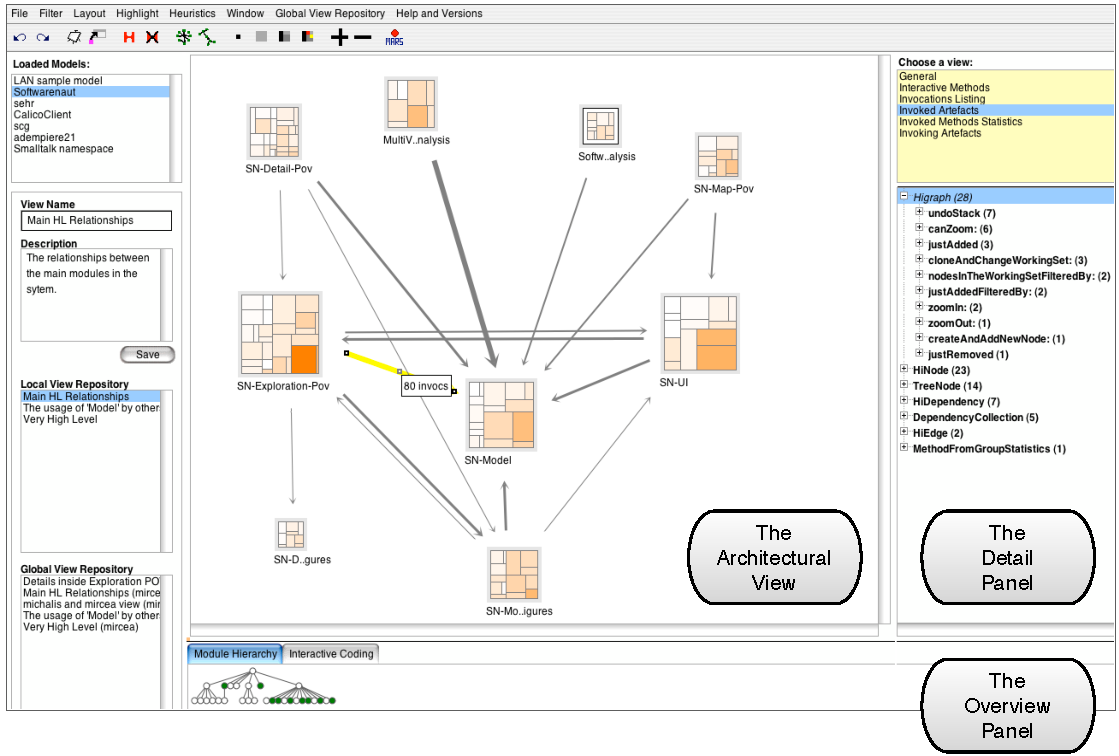
\includegraphics[width=\linewidth]{SnautOnSnaut.pdf}
\caption{Softwarenaut uses linked views to present multiple perspectives on a software system at once}
\flabel{sos}
\end{center}
\end{figure}

The UI of Softwarenaut contains three linked complementary visual perspectives that present information about the system during the exploration. \fref{sos} presents Softwarenaut visualizing an architectural view of itself. The figure illustrates the three complementary views that the tool supports:

\begin{enumerate}

\item The {\em Exploration} panel is Softwarenaut's main view. It is a graph-based representation of modules and their dependencies. The nodes in the graph represent modules and the edges represent the dependencies between the modules. Each dependency edge is an aggregation of low-level dependencies between the two associated modules. To represent the nodes and edges we use Lanza's polymetric approach \cite{lanza-pv, lanza-oomp}. 

\item The {\em Detail} panel presents details for an entity selected in the Exploration panel. The goal is to supplement details of the element selected in the exploration panel. The detail panel implements the ``details-on-demand'' part of Shneiderman's visualization mantra \cite{shneid-eyes}.

\item The {\em Overview} panel presents the entire hierarchy of a system and highlights the modules that are visible in the exploration panel. The Overview panel presents a horizontal slice through a system \cite{wong-thesis}, offering an orientation aid which is critical for successful navigation \cite{storey-awareness}.

\end{enumerate}

Like other architecture recovery tools \cite{pollet-sar}, Softwarenaut conforms to a classical extract-abstract-view architecture. 

\begin{figure}[h]
\begin{center}
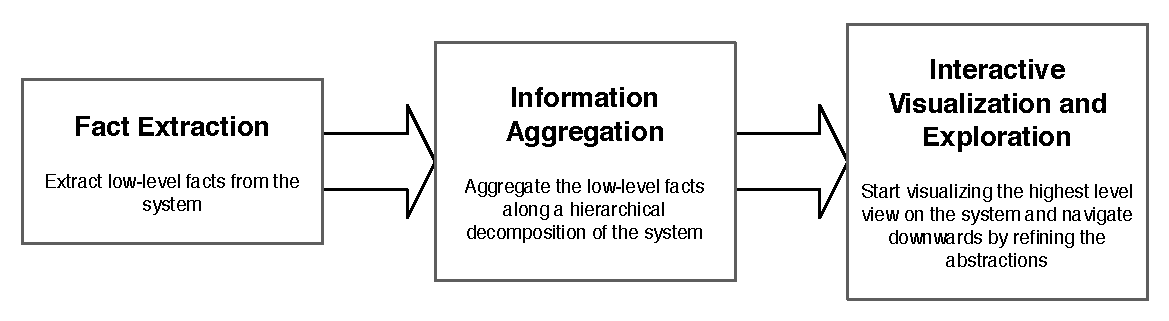
\includegraphics[width=\linewidth]{SnautFlow}
\caption{Softwarenaut supports an extract-abstract-view workflow model}
\flabel{flow}
\end{center}
\end{figure}

\fref{flow} presents the three main steps of this architecture, {\em fact extraction}, {\em information aggregation}, and {\em interactive visualization and exploration}, which we detail in the next sections.

\newpage

%%%%%%%%%%%%%%%%%%%%%%%%%%%%%%%%%%%%%
%%%%%%%%%%%%%%%%%%%%%%%%%%%%%%%%%%%%%
\section {Fact Extraction and Modelling} \label{sec:facts}
%%%%%%%%%%%%%%%%%%%%%%%%%%%%%%%%%%%%%
%%%%%%%%%%%%%%%%%%%%%%%%%%%%%%%%%%%%%

At the lowest level, Softwarenaut models a system using the Core of the FAMIX meta-model \cite{tichelaar-thesis}, a language independent meta-model that describes the static structure of object-oriented software systems. 

%%%%%%%%%%%%%%%%%%%%%%%%%%%%%%%%%%%%%
\subsection {Entities and relationships in FAMIX}
%%%%%%%%%%%%%%%%%%%%%%%%%%%%%%%%%%%%%

FAMIX represents both artifacts and relationships as first-class entities. The main artifacts are namespaces, packages, classes, attributes, methods, fields. The main relationships between these entities are method invocations, variable accesses, class inheritances, and package include relationships \cite{tichelaar-thesis}.

A class of relationships which have a special importance in Softwarenaut are the containment relationships which organize a software system in a vertical hierarchy: classes contain methods, modules contain classes, systems contain modules. This containment mechanism is a powerful way of coping with the complexity of large software systems.

At an architectural level, different languages provide different mechanisms for the hierarchical organization of the system. C/C++ developers use the directory structure to organize systems hierarchically; Java developers use the package hierarchy; Smalltalk developers use the bundles hierarchy, etc. 

When a hierarchical decomposition is not provided, we can automatically generate one using clustering techniques \cite{koschke-thesis}. We presented elsewhere an experiment with clustering the classes in a system based on natural language similarity\cite{Lung05a}.

%%%%%%%%%%%%%%%%%%%%%%%%%%%%%%%%%%%%%
\subsection {Language Independence}
%%%%%%%%%%%%%%%%%%%%%%%%%%%%%%%%%%%%%

Given that the FAMIX meta-model is language independent, Softwarenaut can analyze any system written in an object-oriented language. This requires fact extractors that analyze the source code and build the intermediary FAMIX model. For this we use various third-party tools like McC \cite{pepi-mcc} or inFusion\footnote{See \url{http://www.intooitus.com/inFusion}, verified Jan 25 2011.}.

\newpage

%%%%%%%%%%%%%%%%%%%%%%%%%%%%%%%%%%%%%
%%%%%%%%%%%%%%%%%%%%%%%%%%%%%%%%%%%%%
\section {Information Abstraction} \label{sec:org}
%%%%%%%%%%%%%%%%%%%%%%%%%%%%%%%%%%%%%
%%%%%%%%%%%%%%%%%%%%%%%%%%%%%%%%%%%%%

Aggregating horizontal relationships between software artifacts along the containment relationships is the fundamental technique that enables abstraction in Softwarenaut. 

\fref{dep-agg} exemplifies the aggregation of low-level relationships between methods and classes along the containment hierarchy of a Java system. 

\begin{figure}[ht]
\begin{center}
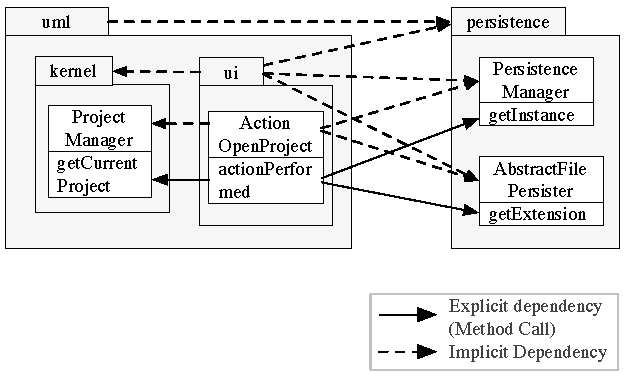
\includegraphics[width=\linewidth]{DependencyAggregation}
\caption{The aggregation of explicit dependencies into implicit ones along the containment relationships between methods, classes, and packages in a Java system}
\flabel{dep-agg}
\end{center}
\end{figure}

The example contains two explicit low-level dependencies: the method calls between \cod{mc1} and respectively \cod{mc2} and \cod{mc5}. The explicit dependencies propagate as implicit relationships vertically along the containment relationships \cod{mc1 $\rightarrow$ c1 $\rightarrow$ B  $\rightarrow$A}, \cod{mc5 $\rightarrow$ c5 $\rightarrow$ d $\rightarrow$ c} and \cod{mc2 $\rightarrow$  c2 $\rightarrow$  d $\rightarrow$ c}. The highest level implicit relationship is the one between A and C. 

A data structure that allows for this is the Higraph introduced by Harel \cite{harel-visform}. In our case, the DPMHigraph\footnote{DPM stands for Detail Project Model} is a data structure formed by taking the graph of basic artefacts and relationships between them and aggregating them along the containment hierarchy of the system. 

\begin{figure}[h]
\begin{center}
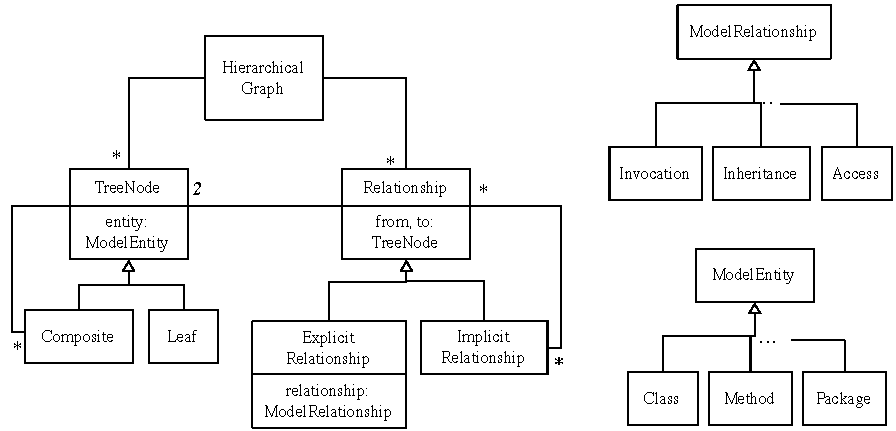
\includegraphics[width=0.9\linewidth]{HigraphModel}
\caption{The DPMHigraph model is the core representation of a system in Softwarenaut}
\flabel{hmodel}
\end{center}
\end{figure}

The diagram from \fref{hmodel} presents two types of abstract entities and two types of abstract relations:

\begin{itemize}

\item {\em Leaf Entities}. They are the basic object-oriented programming building blocks used for the structuring of software. Depending on the analyzed relationship, the leaf entities can be either methods or classes.

\item {\em Composite Entities}. The composite entities are containers for other entities. They can have direct mappings to programming language entities, such as classes, packages, namespaces or modules but can also represent abstract composites such as clusters.

\item {\em Explicit Relationships}. These are the relations between two entities as they exist in the code. Softwarenaut models method invocations, class inheritance, and field access.

\item {\em Implicit Relationships}. The model admits relationships between any abstract entities. However, in software systems explicit relationships usually exist only between the leaf entities. Therefore, the relations between the composite entities must be inferred bottom-up from the relations existing between the leafs. The result is that between any two high-level components, we have a relation that represents a collection of all the relations between the leaf components aggregated in them.

\end{itemize}

%%%%%%%%%%%%%%%%%%%%%%%%%%%%%%%%%%%%%
%%%%%%%%%%%%%%%%%%%%%%%%%%%%%%%%%%%%%
\section {Interactive Exploration} \label {sec:interact}
%%%%%%%%%%%%%%%%%%%%%%%%%%%%%%%%%%%%%
%%%%%%%%%%%%%%%%%%%%%%%%%%%%%%%%%%%%%

In this section we detail the interactive techniques that support the exploration process in Softwarenaut: navigation (\ref{sec:navi}), details-on-demand (\ref{sec:dod}), rule-based filtering (\ref{sec:filtering}) and first-class views (\ref{sec:views}).  

%%%%%%%%%%%%%%%%%%%%%%%%%%%%%%%%%%%%%
\subsection{Navigation} \slab{navi}
%%%%%%%%%%%%%%%%%%%%%%%%%%%%%%%%%%%%%

The dominant exploration mechanism of Softwarenaut is navigation along the vertical decomposition of the system. One starts with a very high-level abstracted view of a system and continuously refines by using exploration operations \cite{robertson-conetrees}. At any given moment the set of visible nodes in the exploration view with which the user interacts constitutes the working set (WS). Initially the working set contains very few high-level nodes. As the user explores the system he transforms the working set by performing exploration operations on it and thus changes the contents of the view in the exploration view.

\begin{figure}[ht]
\begin{center}
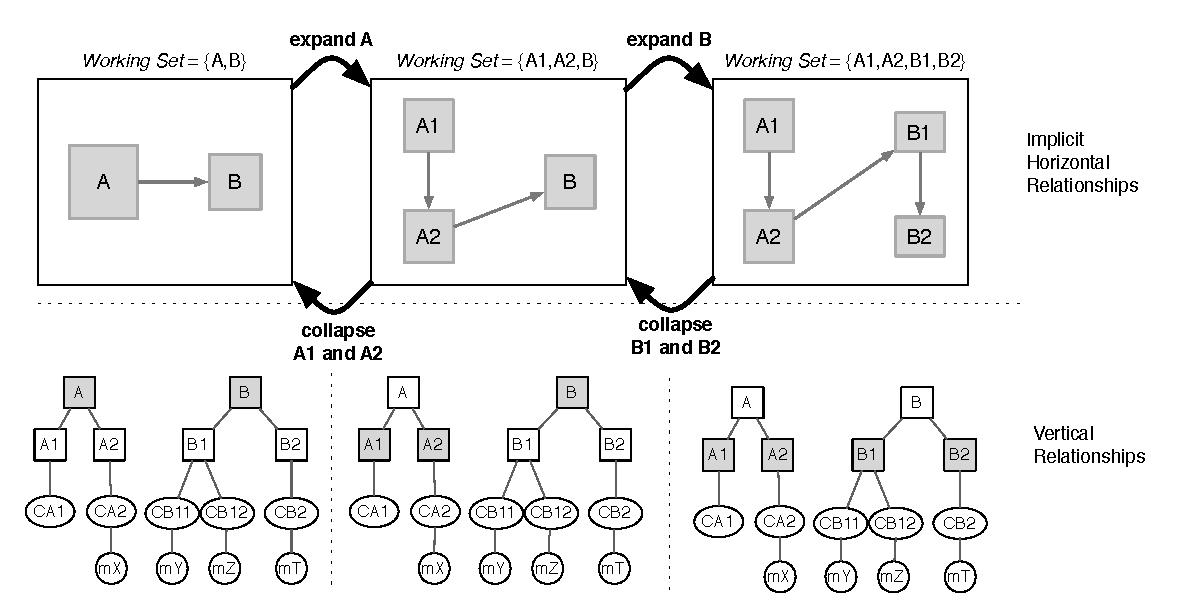
\includegraphics[width=\linewidth]{SnautSequence}
\caption{The expand and collapse complementary operations that allow vertical navigation in the Higraph}
\label{}
\end{center}
\end{figure}

The exploration operations supported by Softwarenaut are:

\begin{itemize}

\item {\em Expand}. The expand operation applied to a node of the working set replaces in the working set the node with nodes that represent its children. We define the operation formally as follows: 

$ Expand_{N,HG} (WS) = WS - N + children (N, HG)$, 

where $children(x,h)$ is a function which returns the children of node $x$ in higraph $h$.

\item {\em Collapse}. The collapse operation applied to a module in the working set removes the module and all its siblings from the view and replaces them with their parent module. We define the operation as follows:

$ Collapse_{N,HG} (WS) = WS - N - siblings (N, HG) + parent (N, HG)$

where $siblings(x,h)$ is a function which returns the nodes that have the same parent with $x$ in higraph $h$, and $parent(x,h)$ is a function which returns the parent of node $x$ in higraph $h$. 

\item {\em Filter}. The filter operation applied to a node removes that node from the working set. We define the operation as follows:

$ Filter_{N,HG} (WS) = WS - N$

\item {\em Group}. The group operation applied to several modules removes the modules from the view and replaces them with a new virtual module. By grouping several modules together the user reduces the clutter in the view. We define the group operation as follows: 

$ Group_{N_{i},HG} = WS - N_i + NewGroupNode $

where $N_i$ is the set of nodes the user wants to group.

\end{itemize}

As the user refines the view, and climbs down in the hierarchy of the system, he brings more and more elements into the view. He can use the Filter and Group operations on explicit sets of nodes to decrease the number of nodes displayed on screen and therefore cope with the complexity of large graphs. One type of modules that benefit the user when filtered out are the {\em omnipresent modules} which contribute little to the understanding of the architecture of the system, and heavily clutter the view \cite{mitchell-bunch}.

%%%%%%%%%%%%%%%%%%%%%%%%%%%%%%%%%%%%%
\subsection {Details-on-Demand} \slab{dod}
%%%%%%%%%%%%%%%%%%%%%%%%%%%%%%%%%%%%%

The elements of every architectural view in Softwarenaut are nodes that represent modules and edges that represent relationships between them. For the user to be confident that he {\em understands} such a view he needs to understand the role of every node and the meaning of every edge. Metaphorically, if the view were a phrase, the nodes would be the nouns and the edges would be the verbs. Only when one has understood all the nouns and the verbs he has really understood the story of the view.  

The Detail panel of Softwarenaut is one of the ways in which one can understand the individual nodes and edges in an architectural view; it presents different views depending on the selected element in the exploration view. 

%%%%%%%%%%%%%%%%%%%%%%%%%%%%%%%%%%%%%
\subsubsection {Detail Views for Modules}
%%%%%%%%%%%%%%%%%%%%%%%%%%%%%%%%%%%%%

The detail views for modules present various aspects of a selected module. \fref{dnode} presents the {\em Class Metrics} detail view which lists all the classes contained in a module together with a customizable set of metrics for them.

\begin{figure}[ht]
\begin{center}
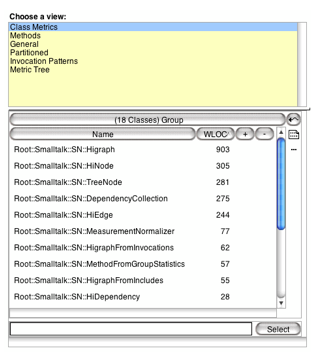
\includegraphics[width=0.5\linewidth]{DetailForNode}
\caption{The Class Metrics view shows the list of classes in a module. The classes are sorted based on their size and the user can navigate to the source of individual classes.}
\flabel{dnode}
\end{center}
\end{figure}

%%%%%%%%%%%%%%%%%%%%%%%%%%%%%%%%%%%%%
\subsubsection {Detail Views for Relationships}
%%%%%%%%%%%%%%%%%%%%%%%%%%%%%%%%%%%%%

The detail views for relationships present information about the selected relationships. Since understanding the relationships is critical for understanding the view, Softwarenaut provides a broad set of detail views for relationships which cover both structural and evolutionary aspects of the relationships \cite{lungu-cutedge, lungu-relevo}. 

\fref{dedge} presents two such examples: to the left is the Invoked Artifacts view and to the right is the Interactive Methods view. 

\begin{figure}[ht]
\begin{center}
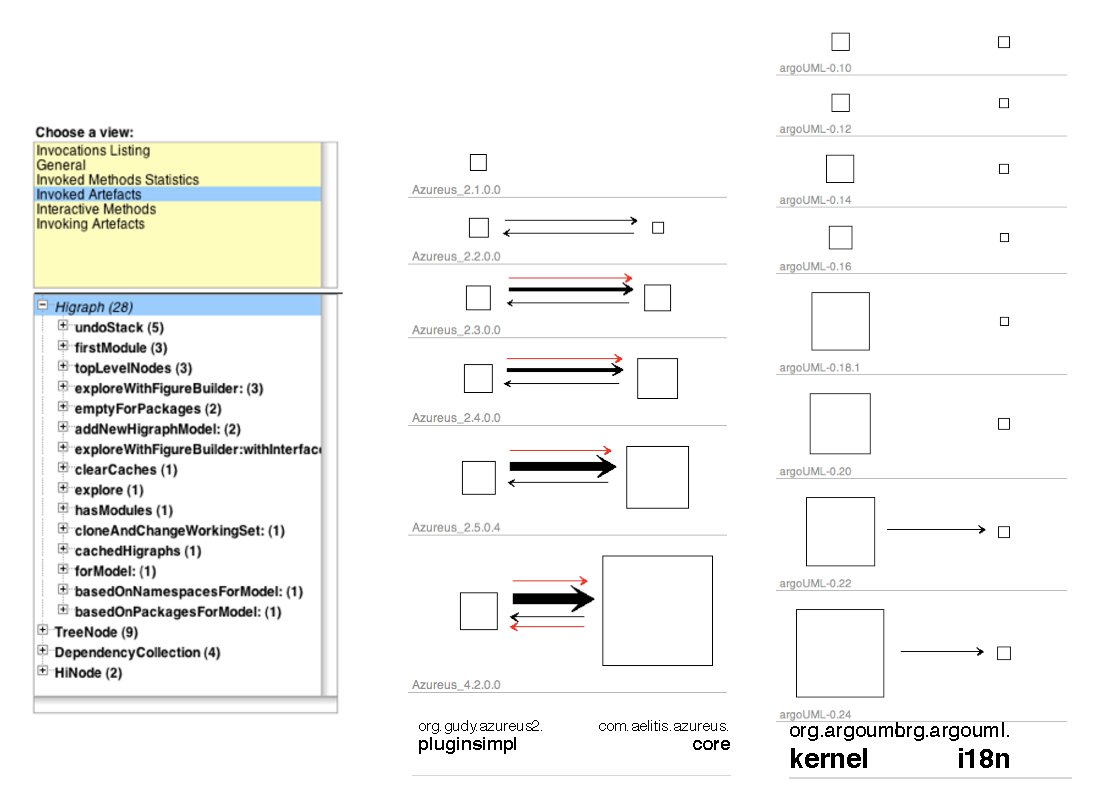
\includegraphics[width=0.8\linewidth]{DetailsForEdge}
\caption{Two example detail views for a relationship: (left) the Invoked Artifacts detail view; (right) the Interactive Methods detail view}
\flabel{dedge}
\end{center}
\end{figure}

The Invoked Artefacts view lists all the artefacts invoked by the selected high-level dependency. The tree has on its first level the names of the invoked classes. The children of every class node are the invoked methods. The method nodes can be further expanded to reveal the call sites. 

The Interactive Methods detail view presents the call graph of the method calls abstracted in the selected high-level dependency. 

%\newpage
\subsection {Rule-Based Filtering}
\slab{filtering}

In the previous section we have introduced the Filter operation which works on explicit sets of nodes. Most software architecture recovery tools offer such a filter operation \cite{aracic-filtering}. Softwarenaut implements several categories of advanced {\em rule-based filters} for nodes and edges. Softwarenaut supports two types of basic filters: 

\begin{enumerate}

\item {\em Low-level filters} act on the higraph itself. They remove from the higraph the low-level elements that match a given condition, e.g., all the invocation relationships that go to polymorphic classes.

\item {\em High-level filters} act on the high-level elements and relationships between them in the working set, e.g., hiding all the high-level dependencies that abstract few low-level dependencies.

\end{enumerate}

During exploration, the user interacts mostly with the High-level filters. There are two types of filters that apply to both artifacts and relationships: 

\begin{enumerate}
\item {\em Metric-based filters} for entities and relationships are defined with respect to the metrics computed for artifacts. For example filtering out {\em the weak dependencies} or {\em the small modules} in a view.
\item {\em Type-based filters} for entities and relationships are defined with respect to the type of the artifacts. For example showing {\em only inheritance relationships} or hiding {\em all the classes} from a view.
\end{enumerate}

Softwarenaut also implements advanced filters for relationships:

\begin{itemize}

\item {\em Evolutionary filters} are defined based on the historical evolution of an inter-module relationship in the system\footnote{Evolution-based filters require models of multiple versions of a system loaded}. For example showing only the {\em relationships that existed in all the versions of a system} or hiding all the {\em unstable relationships} \cite{lungu-relevo}.

\item {\em Directional filters} are defined based on the direction of the relationship between two modules. For example, filtering out the unidirectional relationships from an architectural view is useful for highlighting the modules that have mutual dependencies between themselves. 

\end{itemize}

\begin{figure}[ht]
\begin{center}
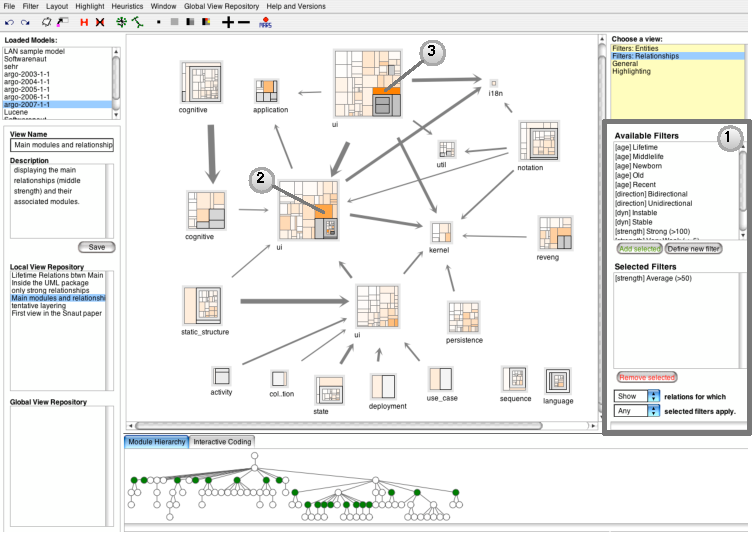
\includegraphics[width=0.9\linewidth]{SnautFilteringPanel}
\caption{The UI for applying relationship filters in Softwarenaut}
\flabel{filpan}
\end{center}
\end{figure}

\fref{filpan} presents the relation filtering panel as implemented in Softwarenaut. Several filters can be combined to obtain more powerful ones with either the ``and'' or the ``or'' operator. The elements that match the filter can be either ``shown'' or ``hidden''. The user can define new filters by writing simple scripts in Smalltalk. The system is fully reflective, and as soon as a new filter is defined, it will immediately appear in the list of available filters.

Rule-based relationships are a powerful way of reducing information in the view. The principle is simple: not all the relationships are equally relevant for the task at hand. When analyzing a system with a specific goal, the analysis focuses first on those relationships that are most relevant for the chosen goal. Two different goals are architecture recovery and architecture quality assessment: 

\begin{itemize}

\item {\em Architecture Recovery.} When recovering the architecture of a system, the lifetime relationships are more relevant. They represent the architectural backbone of the system and their stability over time insures that it is worth analyzing them first.

\item {Architecture Quality Assessment.} When assessing the quality of an architecture, the recent relationships are of higher interest. Since they were recently introduced, they are more likely to be contrary to the original intended architecture. They might be the result of architectural decay or of changes to the system performed by new developers that are unaware of the architecture. Continuously monitoring these relationships can be a good quality assurance policy.
\end{itemize}



\fref{lvr} presents two views on the same modules that are also present in \fref{filpan} but with age-based filters activated. 

\begin{figure}[ht]
\begin{center}
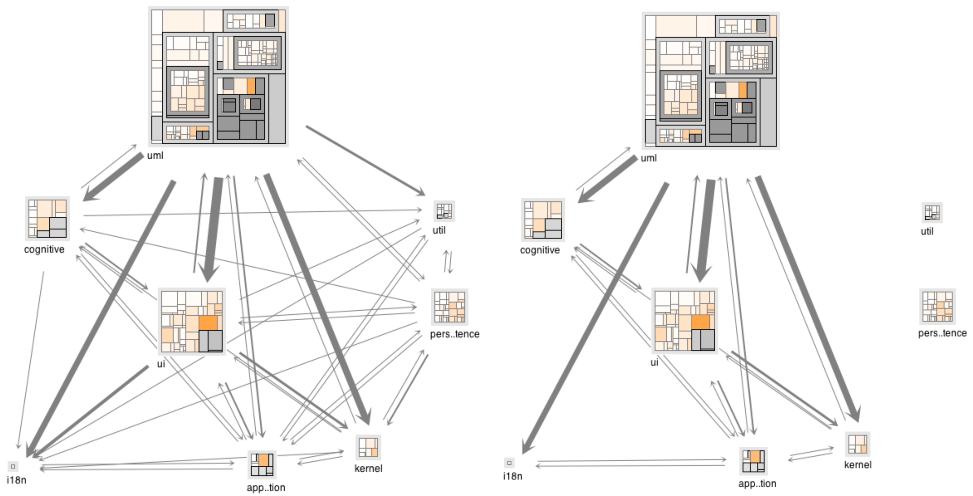
\includegraphics[width=0.9\linewidth]{Architecture-LifetimeVsRecent}
\caption{The left part of the figure shows the Lifetime Relationships while the right part of the figure presents the Recent Relationships in Azureus/Vuze}
\flabel{lvr}
\end{center}
\end{figure}

The left side presents only the Lifetime Relationships - 21 relationships that existed between the displayed modules in all the versions of the system. The right side presents only the Recent Relationships - 36 relationships introduced in the system in the latest version. Both the numbers are very low in comparison with the total number of relationships that are present in the last version of the system; both function as powerful filters.

%\newpage
\subsection {First-Class Views}
\slab{views}

The designers of a system use multiple diagrams for the specification of the architecture of a system. Also the reverse engineers need to recover multiple views when trying to understand the architecture of the system. To avoid information overload, architecture recovery tools usually support some kind of semantic zooming \cite{storey-shrimp}. We address this problem by directing the analysis towards the recovery of multiple architectural views. The technical detail that allows this is view persistence: in Softwarenaut one can save and restore any view during the exploration. This this allows for a {\em divide et impera} approach to architecture recovery and representation: each time a view risks becoming too complex the user saves it and the further exploration focuses only on a sub-part of the view. View persistence requires the following information: The name and version of the system under analysis, the current working set with the positions of all the nodes in it, the active node and edge filters (both explicit and rule based), the creator of the view, and a name and description of the view.

The model of the system is not saved together with the view. We assume that model construction is deterministic and the name and version of the system will suffice for model reconstruction at a later time. % Moreover, in most of the cases the views are reused locally.


%The filters are predefined. In the future we plan to support user-defined filters and their publication together with the views. 

\fref{viops} highlights the way the user can interact with the local views. He has a set of local views that he can save, load, delete locally. 


\newpage
% COLLABORATION
\section {Collaboration}
\label {sec:collab}

% We have shown that in Softwarenaut views are entities that can be saved and restored. In this section we talk about the possibility of sharing the views with other users. 

Once published, a given version of a system never changes. It makes therefore sense to publish all the analyses regarding that version, such that when other users analyze the same version or system they can benefit from the previous work. In the context of architectural view recovery this means discovering architectural views that others have already defined. To support sharing architectural information we have created a {\em Global Architectural View Repository} (GVR) -- a public repository that indexes architectural views \footnote{
Organizations can create their own private view repositories if privacy is a concern}.


As soon as a user starts the analysis of a given system Softwarenaut checks the available view repositories and retrieves the list of views that are already defined for that system and/or version.


\begin{figure}[h]
\begin{center}
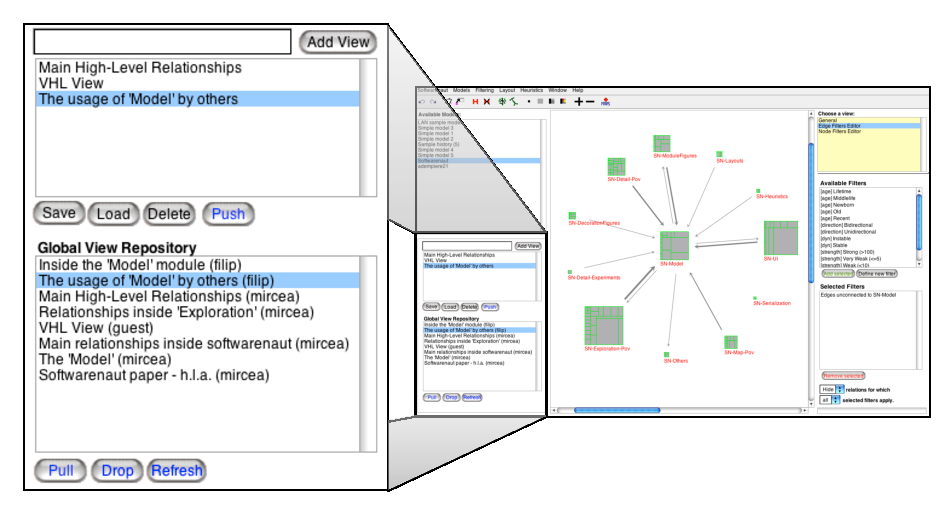
\includegraphics[width=\linewidth]{ViewOperations}
\caption{Views are first-class entities in Softwarenaut. They can be saved, deleted locally, but also published and retrieved from public or private repositories}
\flabel{viops}
\end{center}
\end{figure}

\fref{viops} presents the view UI in Sofwarenaut. The top part of the inset presents the locally stored views which the user can loaded, delete, or push to the GVR. The bottom part presents the views which exist for the given system in the GVR. From the global view repository he can pull views in the local repository, or if he is the creator of such a view he can delete it from the global repository too. The view sharing mechanism is the latest addition to Softwarenaut and we are still waiting to test it with users. 


\subsection {Softwarenaut Synergies}
One of the tools that benefits from the Global View Repository is the Small Project Observatory (SPO), an ecosystem analysis tool that we have introduced elsewhere \cite{lungu-est}. SPO works at an abstraction level above the architectural level of individual systems: the {\em ecosystem abstraction level} \cite{lungu-thesis}. 

\begin{figure}[th!]
\begin{center}
\includegraphics[width=\linewidth]{SpoArchitectural}
\caption{SPO imports architectural views saved in Softwarenaut}
\label{}
\end{center}
\end{figure}
% This type of view is dynamic, it can not become obsolete...

% The main use case in which this navigation is needed is when one wants to understand a given system in the context of the ecosystem. 

SPO needs to support navigation between the two abstraction levels to support the understanding of  the ecosystem abstraction level. When navigating from the ecosystem abstraction level down to the architectural level SPO must present architectural views of the individual systems. When they are available, the architectural views of the individual systems are obtained from the Global View Repository. SPO can therefore reuse architectural information generated with Softwarenaut.

% In such a case SPO allows navigating down to the architectural level of the individual system, where it presents architectural views which are enriched with information from the ecosystem. 



\newpage
% DISC
\section {Discussion}
\label {sec:disc}

\subsection {Evaluating the Usability and Usefulness of the Tool}
We have tested the Softwarenaut tool with students in the Software Evolution master course at the University of Lugano. In a qualitative experiment we asked the students to analyze a large software system they have never seen before with the help of Softwarenaut and to produce an architectural report. We also asked them to fill a post-analysis questionnaire. Our goal in organizing the experiment was to test Softwarenaut and get feedback on both the usability of the tool and its usefulness for architecture recovery in the context of large software systems. 

To make the assignment more engaging for the students we grouped them in teams of two. After the students submitted the reports, we analyzed them ourselves and found them to be of various detail and quality. We observed that every group came with a different perspective and with a set of different views on the system. We considered this to be an argument for supporting multiple views in architecture recovery. From our experiments we could conclude that ``{\em architecture is in the eye of the beholder}'' just as quality \cite{bass-architecture}.

By analyzing the post-experiment questionnaire we made several observations:

\begin{itemize}
\item Most of the students found the tool easy to use 
\item Most of the students considered that the reports they generated were reliable and they got a better understanding of the system by using Softwarenaut
\item The features that the students found most useful in their analysis were the details-on-demand views, and the predefined filters for both nodes and edges.
\item The features that the students thought were missing were: undo/redo facilities, parametrizable filters, arbitrary and rule-based grouping of elements\footnote{Since then we have implemented most of the features that the students requested.}
\end{itemize}

In the future we plan to empirically validate the usefulness of collaboration in architecture recovery and its implementation in the GVR.


\subsection {Integration with the Moose Analysis Platform}
We built Softwarenaut on top of the Moose Analysis Platform \cite{nier-story}. The main feature that the tool uses from Moose is the FAMIX Core meta-model for representing object-oriented systems. The reliance of Softwarenaut on the FAMIX Core meta-model allows it to be independent of the programming language and analyze systems written in any language as long as there is a fact-extractor for that particular language. 

Softwarenaut makes uses of several of the views defined in Moose for the detail panel (e.g. the views that present entity metrics). Also, since behind any visual element of Softwarenaut lays a HiNode and behind it there is a FAMIX entity one can spawn other Moose analyses by selecting any of the elements of a Softwarenaut architectural view. 



\subsection {Beyond Architecture Recovery(I): Reengineering}
One of the tools built on top of Softwarenaut is MARS: an automated architecture refactoring recommender tool \cite{boeckmann-mars}. The tool starts from a given Softwarenaut view and checks whether move operations applied on classes can improve the architecture of the system by increasing coupling and decreasing cohesion. Preliminary results show a good recall but a low precision of the  automated refactoring recommendations generated by MARS. We plan to further study this phenomenon.


\subsection {Beyond Architecture Recovery (II): Monitoring Software Evolution}

One of our future projects is exploring ways in which the recovered views can function as a live documentation of an evolving system. The Softwarenaut views are not simple pictures but instead they code relationships between the modules of the system. A view recovered for a given version of the system can function as a reference point for presenting the future evolution of the system. After the publication of a new version of the system, Softwarenaut can automatically detect the views affected by the new changes, and visualize these changes on them.


\subsection {Installation and Documentation}
Softwarenaut is written in the Smalltalk programming language and is released under the open source MIT Licence. The tool is available online at {\footnotesize \url{http://www.inf.usi.ch/phd/lungu/softwarenaut/}}. On the homepage of the tool there are a set of screencasts that present its various features together with other documentation, installation instructions, and instructions on how to obtain the source code. 


\newpage
% REL
\section {Related Work}
\label {sec:rel}

There is an extended tradition of architecture recovery tools in software engineering research. Pollet et al. have presented a comprehensive overview of the work in architecture recovery in their survey article \cite{pollet-sar}. In this section we take several of the core aspects of Softwarenaut and we discuss how they are similar and how they differ from other state of the art tools.

\subsection {Exploration and Navigation.} Automatically aggregating the low-level relations, and then letting the user navigate from the highest abstraction level downwards is the main interaction approach in Softwarenaut. This is the exact opposite of the approach that M{\"u}ller proposed with Rigi \cite{muller-revengenv}. In their case, the user starts from the lowest-level facts and aggregates them as he climbs up in the abstraction hierarchy. Their approach does not scale when analyzing very large systems because the number of low-level artifacts is too large. Storey took the same top-down navigation approach in her work on SHriMP \cite{storey-shrimp}.

\subsection {Filtering.} 
%Most of the architecture recovery tools support filtering \cite{aracic-filtering}. The majority of the tools allow for the explicit filtering of individual relations. 

As far as we are aware we are the only ones to propose filters based on evolutionary aspects of the relationships in the context of software exploration. However, there are two related works. The first is Wierda et al. who recover the architectural decomposition of a system through clustering; they observe that if they use for clustering only those dependencies that were in the system in both the first and the last versions, the decompositions are more precise \cite{wierda-clustering}; this observation supports our approach of using the lifetime relationships as more architecturally relevant than the other relationships. 

The second related work is of Abram Hindle et al. \cite{hindle-yarn} who introduce the YARN visualization prototype which animates the evolution of dependencies between the modules of a system. The main difference between our approach and theirs is that we work on a snapshot-based model and they work on a commit-based model. Their commit-based model is advantageous since they benefit from more detailed information about the system; the disadvantage is that the animation of all the commits is time consuming. They do not support a query mechanism for visualizing only special types of relations.


\subsection {First-Class Views and Collaboration.} The work of Storey et al. on Shrimp also allows for saving and restoring views \cite{rayside-flow}. The views are saved inside a ``Filmstrip'' which is persistent. Through the intermediation of the filmstrips the users can restore exploration sessions or even share certain views. This type of information allows people that know about each other to share information by emailing the files. The advantage of the Global View Repository is that it allows for discovering information that other users have discovered and about which the analysis is not aware. 
%(http://www.thechiselgroup.org/shrimp_manual_filmstrip)


Relevant for the collaborative reverse engineering part of our work is the Churrasco work of D’Ambros et al. \cite{dambros-churrasco}. Churrasco supports software evolution modeling, visualization and analysis through a web interface. 
Through an example scenario they show that Churrasco allows for collaborative software evolution analysis, and they attribute this to the availability on the web of the tool. The collaboration happens by annotating the various elements in the views of Churrasco. However, their tool presents a set of predefined views and they are not that much architectural views but rather design-level views. 

One project developed with collaboration support as the main goal is the Jazz IDE of IBM \cite{hupfer-jazz}. The goal of the Jazz ``collaborative development environment'' is to enhance and enrich collaboration in small, informal software development teams. Jazz has several features to support awareness of team member activities in addition to screen sharing such as local history of chats that are anchored in the code providing therefore context to the discussions. The main difference between their work and ours is the goal of the project.





% CONC
\section {Conclusions and Future Work}
\label {sec:conc}

In this article we have presented Softwarenaut, our tool which is state of the art in architecture recovery. The tool allows the recovery of architectural views of a software system and supports collaboration and integration with other tools by publicly sharing architectural views.

\vspace{0.5cm}
\footnotesize
{\bf Acknowledgements.} We would like to thank Fabrizio Perin for feedback on this paper.



\newpage

\footnotesize
%% The Appendices part is started with the command \appendix;
%% appendix sections are then done as normal sections
%% \appendix

%% \section{}
%% \label{}

%% References
%%
%% Following citation commands can be used in the body text:
%% Usage of \cite is as follows:
%%   \cite{key}          ==>>  [#]
%%   \cite[chap. 2]{key} ==>>  [#, chap. 2]
%%   \citet{key}         ==>>  Author [#]

%% References with bibTeX database:

\bibliographystyle{model1-num-names}
\bibliography{scg,thesis}
% Authors are advised to submit their bibtex database files. They are
%% requested to list a bibtex style file in the manuscript if they do
%% not want to use model1-num-names.bst.

%% References without bibTeX database:

% \begin{thebibliography}{00}

%% \bibitem must have the following form:
%%   \bibitem{key}...
%%

% \bibitem{}

% \end{thebibliography}


\end{document}

%%
%% End of file `elsarticle-template-1-num.tex'.
